\documentclass[12pt]{article}
	
\usepackage[utf8]{inputenc}
\usepackage[T1]{fontenc}
\usepackage[margin=1in]{geometry}
\usepackage{amsmath}
\usepackage{fancyhdr}
\usepackage{graphicx}
\usepackage{cancel}
\usepackage[spanish,es-tabla]{babel}
\usepackage{hyperref}
\usepackage{listings}
\usepackage{xcolor}

% Configuracion de colores para listings
\definecolor{codegreen}{rgb}{0,0.5,0}
\definecolor{codegray}{rgb}{0.45,0.45,0.45}
\definecolor{codepurple}{rgb}{0.55,0,0.75}
\definecolor{backcolour}{rgb}{0.97,0.97,0.97}

\lstdefinestyle{cstyle}{
    backgroundcolor=\color{backcolour},   
    commentstyle=\color{codegreen}\itshape,
    keywordstyle=\color{blue}\bfseries,
    numberstyle=\tiny\color{codegray},
    stringstyle=\color{codepurple},
    basicstyle=\ttfamily\footnotesize,
    breakatwhitespace=false,         
    breaklines=true,                 
    captionpos=b,                    
    keepspaces=true,                 
    numbers=left,                    
    numbersep=7pt,                  
    showspaces=false,                
    showstringspaces=false,
    showtabs=false,                  
    tabsize=4,
    frame=single,
    rulecolor=\color{black!30}
}
\lstset{style=cstyle}

%%%%%%%%%%%%%%%%%%%%%%
% Configuracion Encabezado / Pie de pagina
\pagestyle{fancy}
\fancyhead[LO,L]{Estructura de Datos}
\fancyhead[CO,C]{FINESI}
\fancyhead[RO,R]{\today}
\fancyfoot[LO,L]{}
\fancyfoot[CO,C]{\thepage}
\fancyfoot[RO,R]{}
\renewcommand{\headrulewidth}{0.4pt}
\renewcommand{\footrulewidth}{0.4pt}
%%%%%%%%%%%%%%%%%%%%%%

\begin{document}

\noindent \textbf{Universidad Nacional del Altiplano}\\
\textbf{Facultad de Ingeniería Estadística e Informática}\\
\textbf{Docente:} Fred Torres Cruz\\
\textbf{Curso:} Estructura de Datos (2026)\\
\textbf{Autor:} .........\\

\vspace{3mm}
\noindent\textbf{\Large Trabajo Encargado - N° 001}\\
\noindent\textbf{\large Capítulo I: Ejercicios}
\vspace{4mm}
\hrule
\vspace{6mm}

% ==============================================================================
% EJERCICIO 1
% ==============================================================================
\section*{Ejercicio 1}

\noindent\textbf{Enunciado:}
\begin{quote}
Desarrolle un programa en C que registre las horas dedicadas por un analista al procesamiento de un conjunto de datos y el costo por hora. Calcule el costo total del procesamiento y muestre un resumen con las horas trabajadas, tarifa aplicada y costo final.
\end{quote}

\noindent\textbf{Código Fuente (C):}
\begin{lstlisting}[language=C]
#include <stdio.h>

int main() {
    float horas;
    float costo_por_hora;
    
    printf("Ingrese las horas dedicadas: ");
    scanf("%f", &horas);
    
    printf("Ingrese el costo por hora: ");
    scanf("%f", &costo_por_hora);
    
    float costo_total = horas * costo_por_hora;
    
    printf("\n--- Resumen ---\n");
    printf("Horas trabajadas: %.2f\n", horas);
    printf("Tarifa aplicada: $%.2f\n", costo_por_hora);
    printf("Costo final: $%.2f\n", costo_total);
    
    return 0;
}
\end{lstlisting}

\noindent\textbf{Ejecución en Consola:}
\begin{center}
    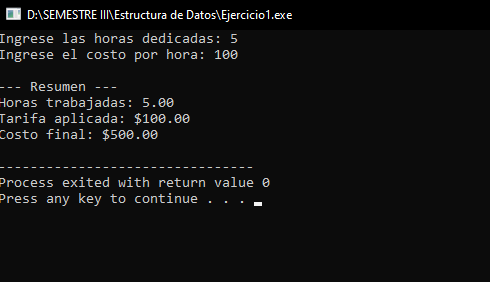
\includegraphics[width=0.72\textwidth]{Ejercicio1-Cmd.png}
\end{center}

\vspace{4mm}
\hrule
\vspace{4mm}

% ==============================================================================
% EJERCICIO 2
% ==============================================================================
\section*{Ejercicio 2}

\noindent\textbf{Enunciado:}
\begin{quote}
Desarrolle un programa en C que registre información básica de una observación de un conjunto de datos: identificador, edad, valor promedio de una variable, categoría representada por una letra y estado de validez del registro. Utilice tipos de datos apropiados y muestre la información almacenada.
\end{quote}

\noindent\textbf{Código Fuente (C):}
\begin{lstlisting}[language=C]
#include <stdio.h>
#include <stdbool.h>

int main() {
    int identificador = 101;
    int edad = 25;
    float valor_promedio = 78.5;
    char categoria = 'A';
    bool estado_validez = true;
    
    printf("--- Informacion de la Observacion ---\n");
    printf("Identificador: %d\n", identificador);
    printf("Edad: %d\n", edad);
    printf("Valor Promedio: %.2f\n", valor_promedio);
    printf("Categoria: %c\n", categoria);
    printf("Estado de Validez: %s\n", estado_validez ? "Valido" : "Invalido");
    
    return 0;
}
\end{lstlisting}

\noindent\textbf{Ejecución en Consola:}
\begin{center}
    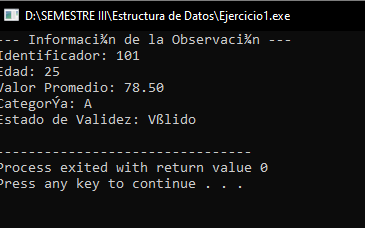
\includegraphics[width=0.60\textwidth]{Ejercicio2-Cmd.png}
\end{center}

\vspace{4mm}
\hrule
\vspace{4mm}

% ==============================================================================
% EJERCICIO 3
% ==============================================================================
\section*{Ejercicio 3}

\noindent\textbf{Enunciado:}
\begin{quote}
Desarrolle un programa en C que solicite una medición decimal obtenida por un sensor, por ejemplo 18.9, la convierta explícitamente a un valor entero y muestre ambos resultados. Indique mediante la salida del programa cuánto valor decimal se pierde durante la conversión.
\end{quote}

\noindent\textbf{Código Fuente (C):}
\begin{lstlisting}[language=C]
#include <stdio.h>

int main() {
    float medicion;
    
    printf("Ingrese la medicion decimal del sensor (ej. 18.9): ");
    scanf("%f", &medicion);
    
    int medicion_entera = (int)medicion;
    float parte_decimal_perdida = medicion - (float)medicion_entera;
    
    printf("\n--- Resultados de la Medicion ---\n");
    printf("Medicion original (decimal): %.4f\n", medicion);
    printf("Medicion convertida (entero): %d\n", medicion_entera);
    printf("Valor decimal perdido durante la conversion: %.4f\n", parte_decimal_perdida);
    
    return 0;
}
\end{lstlisting}

\noindent\textbf{Ejecución en Consola:}
\begin{center}
    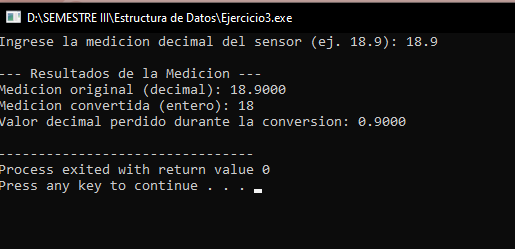
\includegraphics[width=0.72\textwidth]{Ejercicio3-Cmd.png}
\end{center}

\end{document}